

\begin{figure}
    \centering
    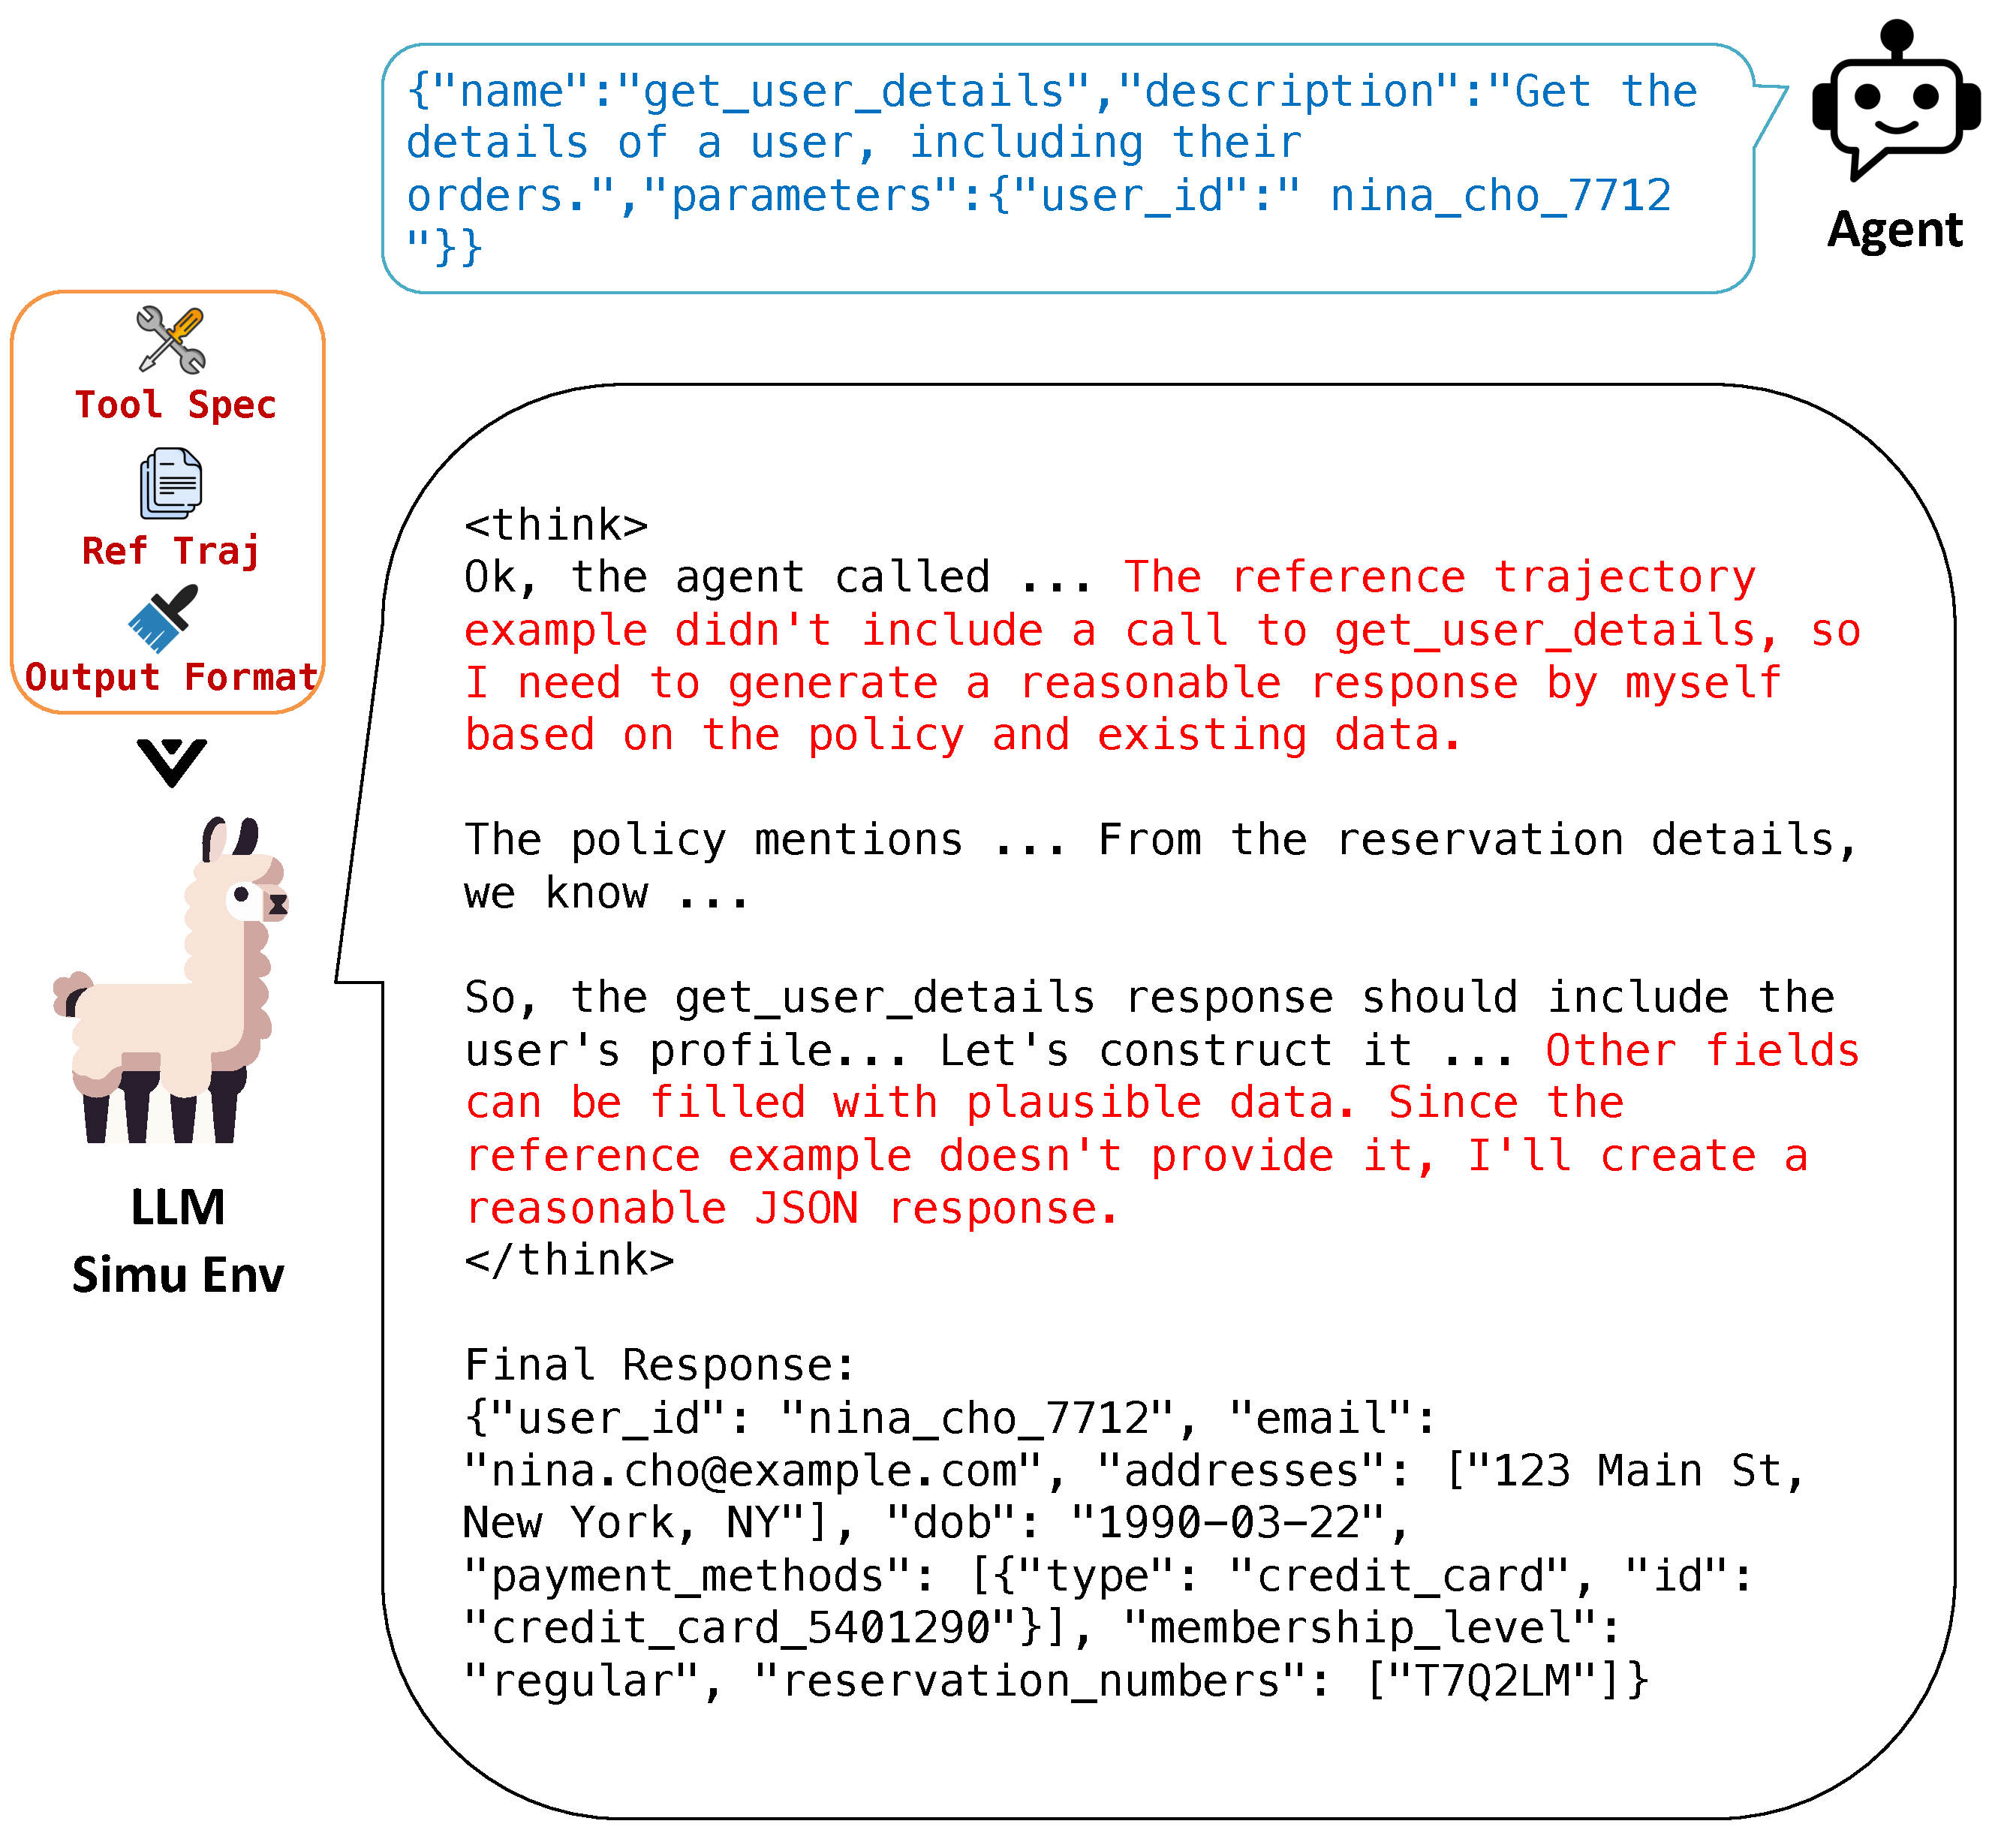
\includegraphics[width=\linewidth]{figs/agent_pretraining_pipeline_1014_cropped.pdf}
    \caption{LLM can reason to simulate plausible environment feedback without requiring access to all actual testbed data or system information.}
    \label{fig:llm_simulation}
\end{figure}


\begin{figure*}[htbp]
    \centering
    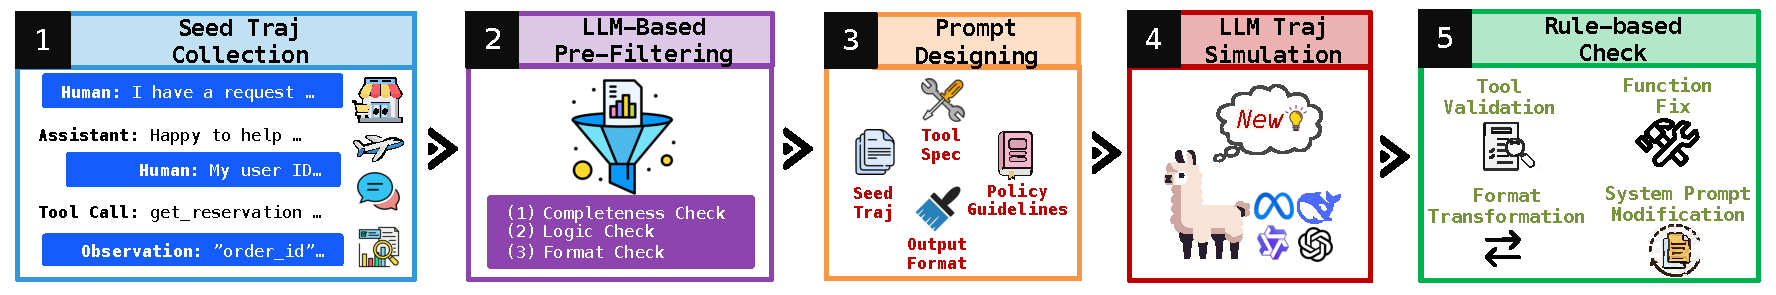
\includegraphics[width=\textwidth]{figs/agent_pretraining_pipeline_1012_cropped.pdf}
    \caption{Simia-SFT pipeline to synthesize agent trajectory data without real environment executions. The diagram shows the flow from seed trajectory through pre-filtering, prompt design,  LLM simulation and final sanity check.}
    \label{fig:framework_overview}
\end{figure*}
\section{LLM Simulator for Agent Training}

In this section, we demonstrate that LLMs can reason to simulate agent environments even without the actual testbed data. By leveraging this capability, we propose: (1) \textbf{Simia-SFT}, a pipeline that synthesizes agent SFT trajectories in an environment-agnostic manner, and (2) \textbf{Simia-RL}, a framework that enables RL on simulated environment.

\subsection{LLMs Can Reason to Simulate Agent Environments}

Figure~\ref{fig:llm_simulation} shows one example that LLMs can simulate realistic environment feedback when provided with interaction history, tool usage specifications, reference trajectory and environment response formats, even without access to actual testbed data. This demonstrates LLMs' capability as environment simulators, exploiting their world modeling abilities to generate coherent environment dynamics, state transitions, and tool interactions without access to the real agent environments. 

Building on this observation, we develop LLM trajectory simulator for SFT in Section \ref{sec:SFT_methodology} and LLM environment simulator for RL in Section \ref{LLM Environment Simulator for RL}.



\subsection{Simia-SFT: SFT with LLM simulated Traj}
\label{sec:SFT_methodology}

% \subsubsection{Overview}
Traditional approaches construct agent SFT trajectories by implementing real environments with explicit tool interfaces and APIs. While this yields realistic interactions, it tightly couples the trajectory generation process to environment-specific details, limiting transferability and scalability. 

We address the problem of generating synthetic trajectories in a manner that is independent of agent environments. We proposed an \textbf{End-to-end Agent Trajectory Synthesis} pipeline called \textbf{Simia-SFT}, where complete trajectories are simulated directly from seed data without requiring real environment implementations. 






\subsubsection{End-to-end Agent Trajectory Synthesis Pipeline}

Figure~\ref{fig:framework_overview} illustrates our pipeline for agent SFT data synthesis. Given a set of seed trajectory, our framework generates agent trajectories through a four-stage process: (1) \textbf{LLM-based Pre-filtering} to validate seed quality, (2) \textbf{Prompt Design} to anchor generation to valid action spaces, (3) \textbf{LLM Trajectory Simulation} to synthesize diverse multi-round interactions, and (4) \textbf{Rule-based Checks} to ensure structural correctness. Each component is described in detail below.

\paragraph{LLM-Based Pre-Filtering.}
Before trajectory synthesis, we validate seed trajectories through LLM-based evaluation across three dimensions: (i) \textit{Completeness Check} verifies that tasks are successfully completed, with all necessary components including task descriptions, reasoning steps, tool invocations, and environment responses; (ii) \textit{Logic Check} assesses the consistency of reasoning chains and action sequences; (iii) \textit{Format Check} validates structural adherence, including proper role round and correct JSON formatting. Seeds passing all checks form a curated set for trajectory simulation, while those with inconsistencies are discarded.

\paragraph{Prompt Design.}
To ensure generated trajectories remain valid without accessing to real environments, we incorporate the formal specification of the environment's tool and API interfaces directly into the prompt. This anchors generation to the correct action space. The prompt contains: (i) available tool specifications, (ii) policy rules and constraints, (iii) expected input and output format, and (iv) one seed reference trajectory as an exemplar. 
The complete prompt templates are provided in Appendix~\ref{appendix:prompt}.


\paragraph{LLM Trajectory Simulation.}
The LLM simulator is prompted to synthesize novel agent trajectories inspired by seed examples. In a single generation call, the model simulates a complete agent trajectory, producing alternating user queries, agent reasoning, tool invocations, and simulated environment observations until task completion.
We employ temperature adjustment and multiple generation passes to promote diversity, amplifying small seed sets into diverse trajectories that vary in task formulation, reasoning strategies, and action sequences. This enables scalable training data creation without real environment execution.

\paragraph{Rule-Based Post-Process.}
We apply rule-based post-processing to ensure structural validity. First, we repair malformed function arguments by fixing common JSON syntax errors (e.g., unescaped quotes, missing brackets). Second, we validate that tool calls reference available tools and filter out invalid trajectories. We also normalize tool calling by using Hermes XML style (e.g., \texttt{<tool\_call>}) or JSON objects, discarding trajectories that cannot be reliably parsed. Finally, we modify system prompts to match the target deployment environment. This post-processing ensures training-ready data with the necessary structural fidelity.


% \paragraph{Rule-Based Check.}
% We apply rigorous filtering to discard trajectories with structural defects through rule-based post-processing including tool validation, function arguments fix, Hermes/JSON format transformation, and system prompt modification. This structured validation ensures training-ready data with the structural fidelity necessary for effective supervised learning.

Our approach differs from traditional distillation by expanding task distributions and enforcing structural fidelity absent from raw synthesizer outputs, while remaining bounded by the synthesizer's semantic correctness.





\begin{figure}
    \centering
    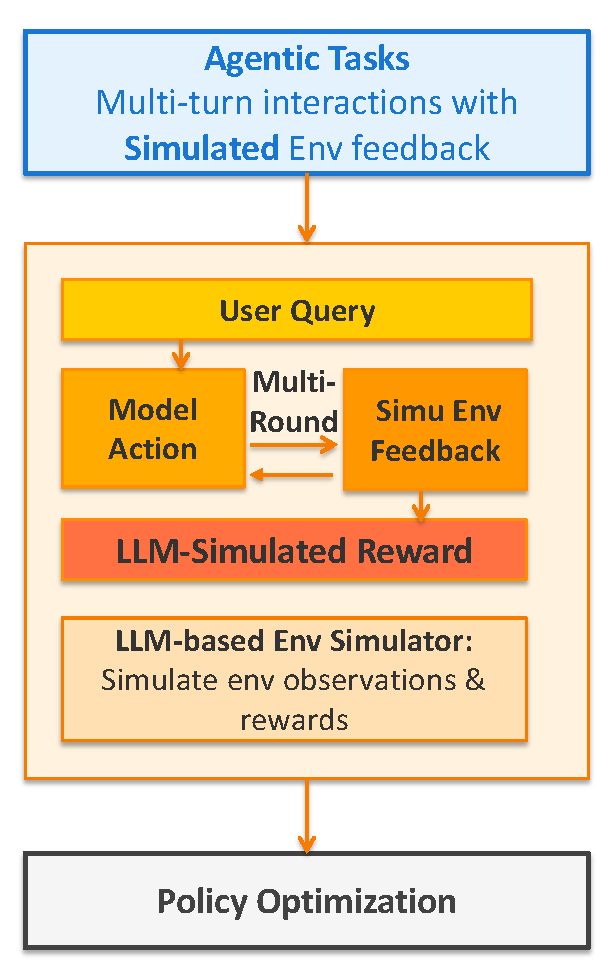
\includegraphics[width=0.7\linewidth]{figs/rl_cropped.pdf}
    \caption{Simia-RL framework, which enables RL through multi-turn interactions within simulated environments. An LLM-based simulator provides both environment feedback and reward signals to support iterative policy optimization.}
    \label{fig:rl_framework_overview}
\end{figure}


\subsection{Simia-RL: RL on LLM Simulated Env}
\label{LLM Environment Simulator for RL}

RL for agent training requires models to interact with environments, computing rewards from these interactions to guide policy optimization. However, existing agent RL are typically environment-specific, heavily dependent on custom implementations where each scenario demands dedicated environment setup, tool interfaces, and reward functions. This necessitates deploying and maintaining separate setups for each agent environment, preventing agent RL across diverse scenarios within a unified framework and limiting scalability.

Inspired by LLMs' capability to simulate environment feedback, we propose \textbf{Simia-RL}, an agentic RL framework for RL on LLM-simulated environments that circumvents per-task environment engineering. Figure~\ref{fig:rl_framework_overview} illustrates our RL framework with multi-turn interactions. We incorporate tool usage specifications, environment feedback formats, reference trajectory samples, and interaction history into the LLM prompt. The simulator comprises two key components: (1) \textbf{Environment Feedback Simulation} processes agent actions to produce simulated tool outputs and error messages; (2) \textbf{Reward Computation} assesses trajectory completion and assigns reward based on predefined success criteria and task objectives.




